\documentclass[journal]{packages/vgtc}                % final (journal style)
%\documentclass[review,journal]{packages/vgtc}         % review (journal style)
%\documentclass[widereview]{packages/vgtc}             % wide-spaced review
%\documentclass[preprint,journal]{packates/vgtc}       % preprint (journal style)
% \documentclass[electronic,journal]{packages/vgtc}     % electronic version, journal

%% Uncomment one of the lines above depending on where your paper is
%% in the conference process. ``review'' and ``widereview'' are for review
%% submission, ``preprint'' is for pre-publication, and the final version
%% doesn't use a specific qualifier. Further, ``electronic'' includes
%% hyperreferences for more convenient online viewing.

%% Please use one of the ``review'' options in combination with the
%% assigned online id (see below) ONLY if your paper uses a double blind
%% review process. Some conferences, like IEEE Vis and InfoVis, have NOT
%% in the past.

%% Please note that the use of figures other than the optional teaser is not permitted on the first page
%% of the journal version.  Figures should begin on the second page and be
%% in CMYK or Grey scale format, otherwise, colour shifting may occur
%% during the printing process.  Papers submitted with figures other than the optional teaser on the
%% first page will be refused.

%% These three lines bring in essential packages: ``mathptmx'' for Type 1
%% typefaces, ``graphicx'' for inclusion of EPS figures. and ``times''
%% for proper handling of the times font family.

% TVCG Packages
\usepackage{mathptmx}
\usepackage{csquotes}
\usepackage{graphicx}
\usepackage{times}

\usepackage{multirow}
\usepackage{booktabs}
\usepackage{amsmath}
\usepackage{caption}
\usepackage{subcaption}
\usepackage[utf8]{inputenc}

% Import other packages
% Extra Packages
\usepackage{url}
\usepackage{epstopdf}
\usepackage{arydshln} % For \hdashline in tables
\usepackage{enumitem} % For [noitemsep] in lists

% Coloring author comments
\usepackage{color}
\usepackage[usenames,dvipsnames]{xcolor}
\definecolor{Purple}{rgb}{.75,0,.85}

\newif\ifnotes
\notestrue
\newcommand{\todo}[1]{\ifnotes {\textcolor{Purple}{\bf TODO: #1\ }} \fi}

% if we want to put in page breaks to assess length
\newif\iftestbreaks
\testbreakstrue
\newcommand{\testbreak}{\iftestbreaks\newpage\fi}

% Useful abbreviations
\usepackage{xspace}
\newcommand{\etal}{\emph{et al.}\@\xspace}
\newcommand{\ie}{\emph{i.e.}\xspace}
\newcommand{\eg}{\emph{e.g.}\xspace}
\newcommand{\etals}{\mbox{\emph{et~al.}'s }}

% TODO NSF CRI / Gleicher commands
\def\naive{na\"{\i}ve}
\def\naively{na\"{\i}vely}

% Droid Sans font
%\usepackage[defaultsans]{droidsans}
%\renewcommand*\familydefault{\sfdefault} %% Only if the base font of the document is to be typewriter style
%\usepackage[T1]{fontenc}
%\linespread{1.1}


% Import Figures
% \newcommand\testfigure{

% \begin{figure}
%   \centering
%   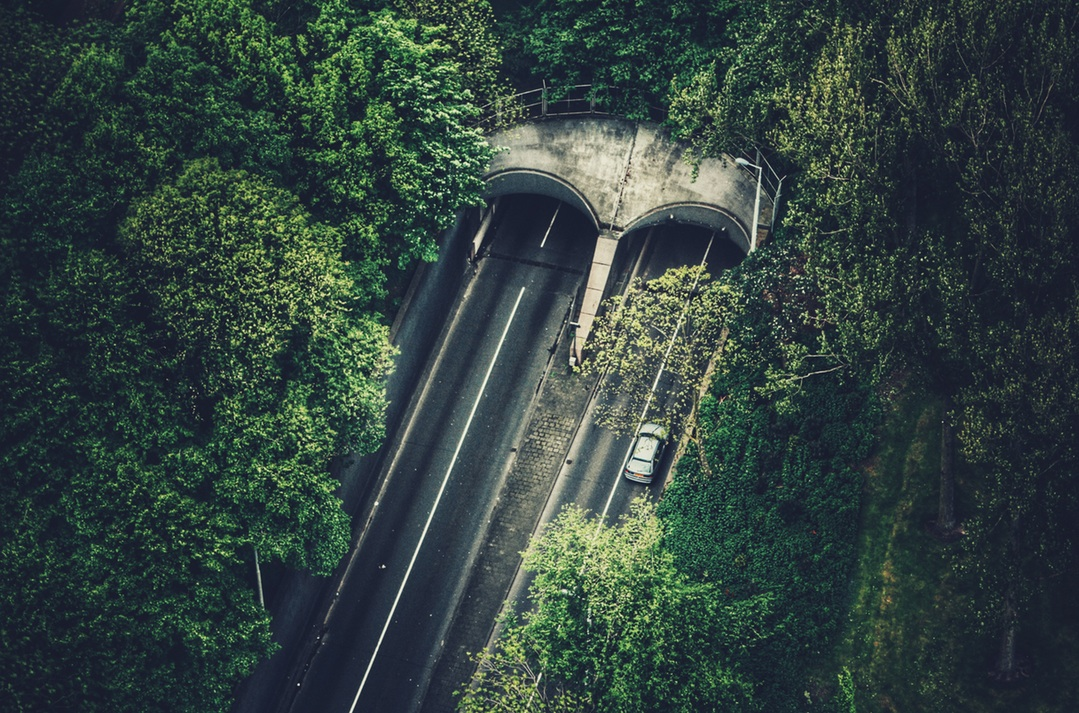
\includegraphics[width=\columnwidth]{img/test}
%   \caption{
%     Please see \S\ref{sec:conclusion}.
%   }
%   \label{fig:protein-validate}
% \end{figure}

% }

\newcommand\guessAError{
  \begin{figure}
    \centering
    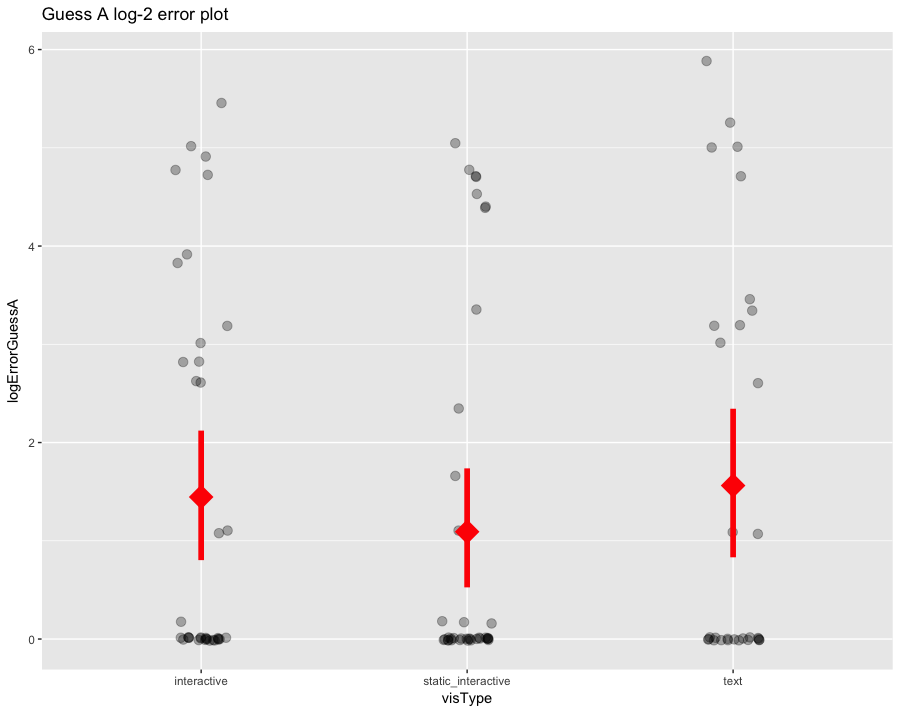
\includegraphics[width=\columnwidth]{img/logError-guessA-104}
    \caption{
      Log error of first lab experiment question.
    }
    \label{fig:guessAErr}

  \end{figure}
}

\newcommand\guessBError{
  \begin{figure}
    \centering
    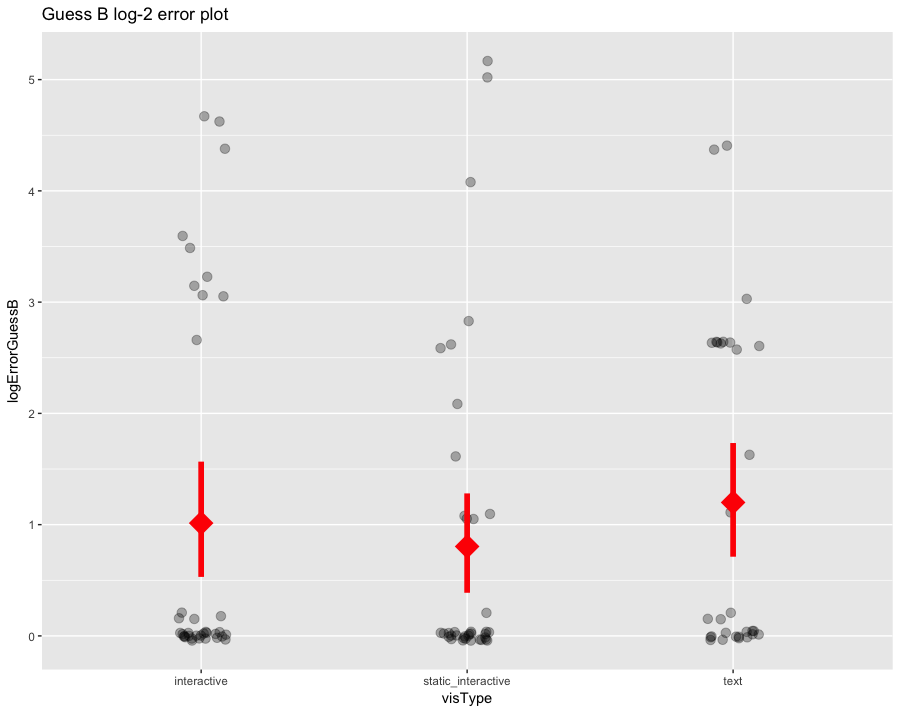
\includegraphics[width=\columnwidth]{img/logError-guessB-104}
    \caption {
      Log error of the second experiment question
    }
    \label{fig:guessBError}
  \end{figure}
}

\newcommand\accuracyPlot{
  \begin{figure}
    \centering
    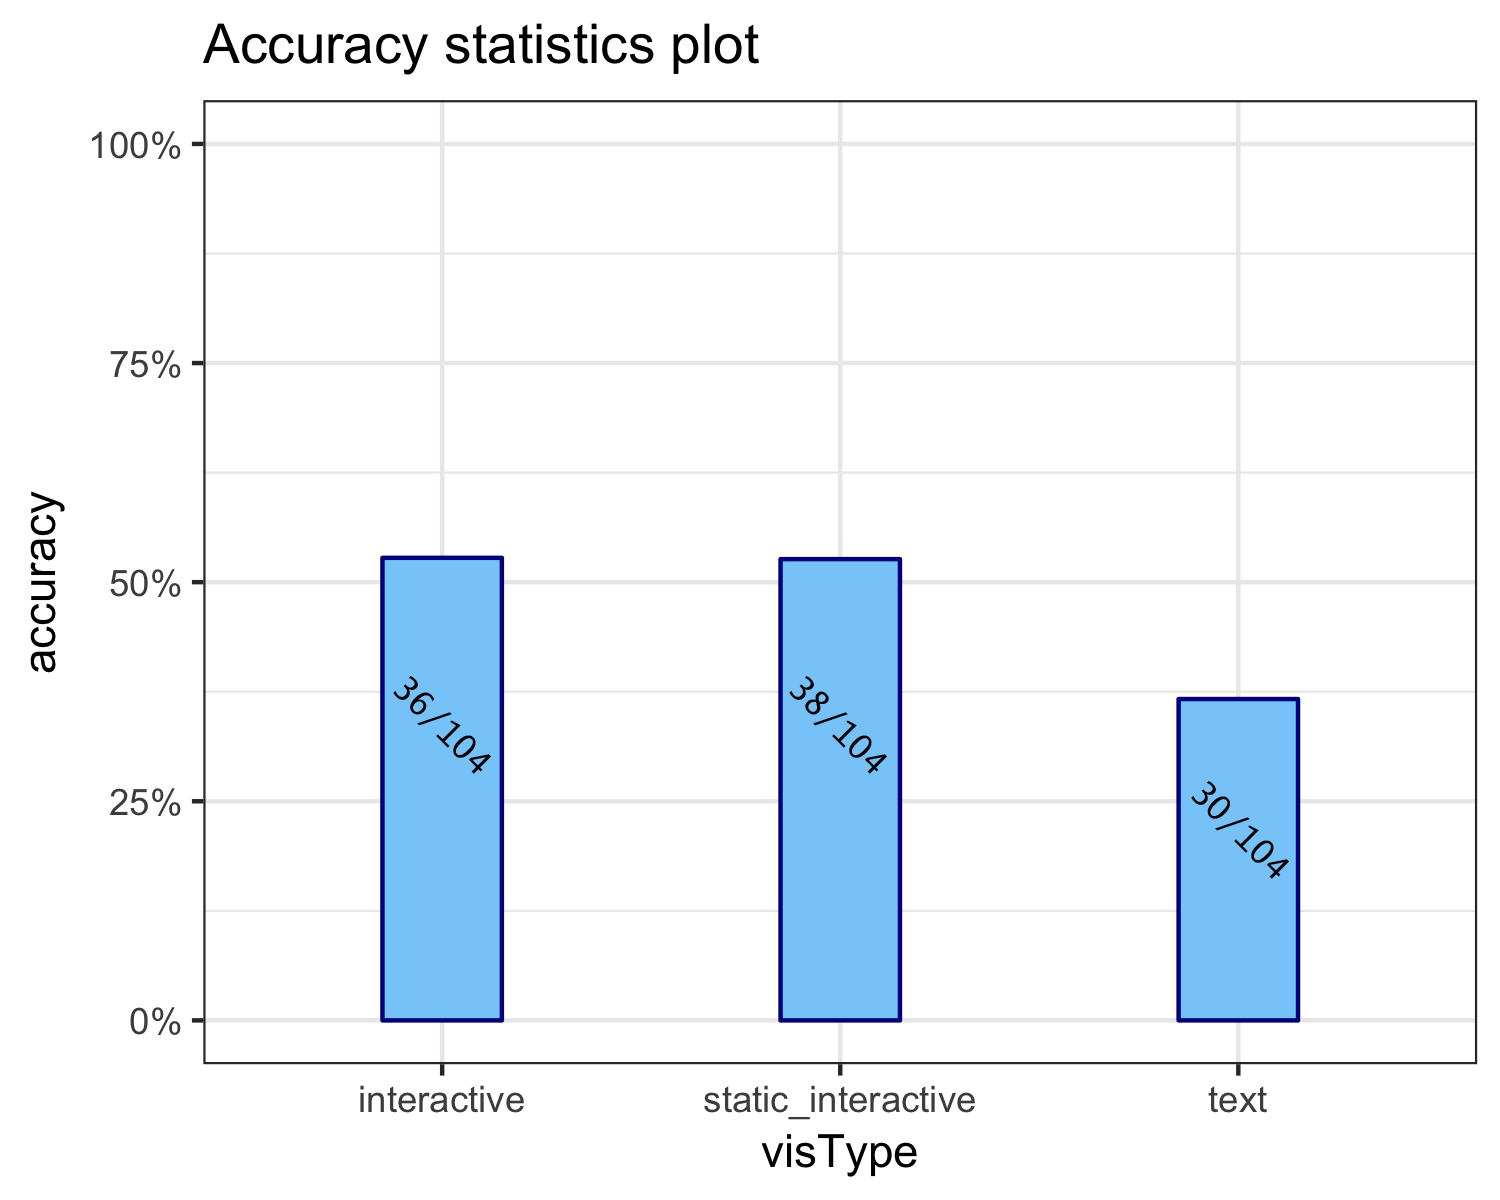
\includegraphics[width=\columnwidth]{img/Accuracy-edit}
    \caption {
      Overall accuracy by visualization type
    }
    \label{fig:accuracyPlot}
  \end{figure}
}

\newcommand\educationAccuracy{
  \begin{figure}
    \centering
    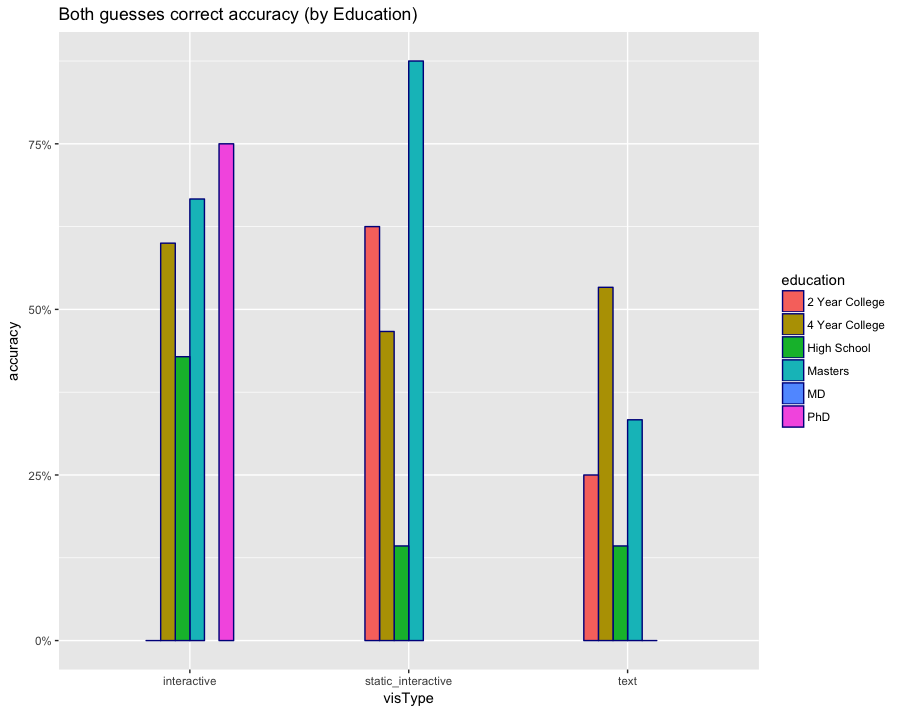
\includegraphics[width=\columnwidth]{img/bothGuessesCorrect-accuracy-byEducation-104}
    \caption {
      Overall accuracy by participants' education
    }
    \label{fig:educationAccuracy}
  \end{figure}
}

\newcommand\experienceAccuracy{
  \begin{figure}
    \centering
    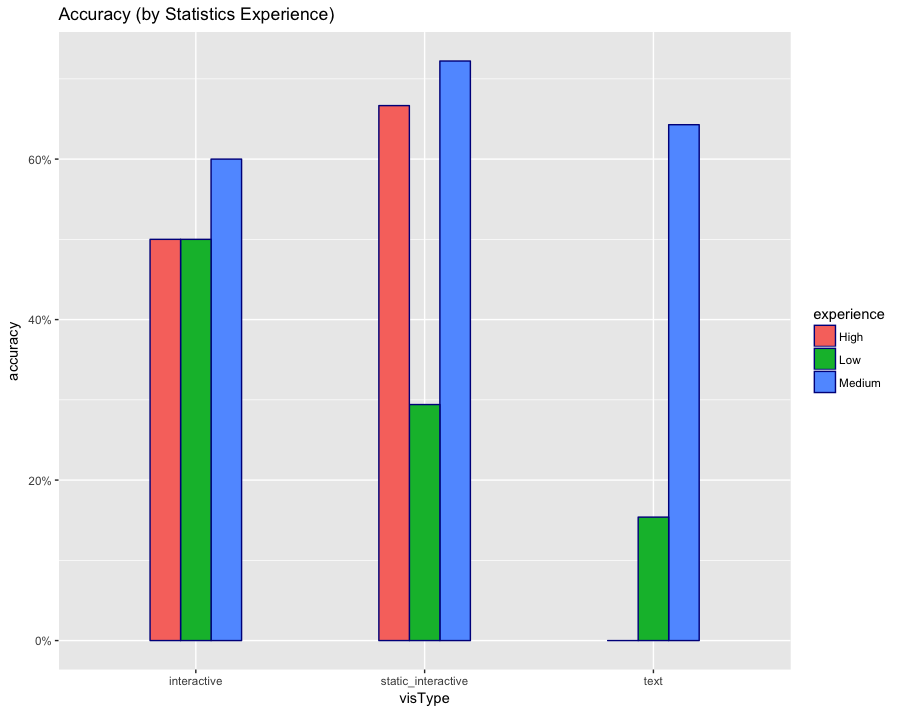
\includegraphics[width=\columnwidth]{img/bothGuessesCorrect-accuracy-byStatExp-104}
    \caption {
      Overall accuracy by participants' statistical experience
    }
    \label{fig:experienceAccuracy}
  \end{figure}
}

\newcommand\interactiveVis{
  \begin{figure}
    \centering
    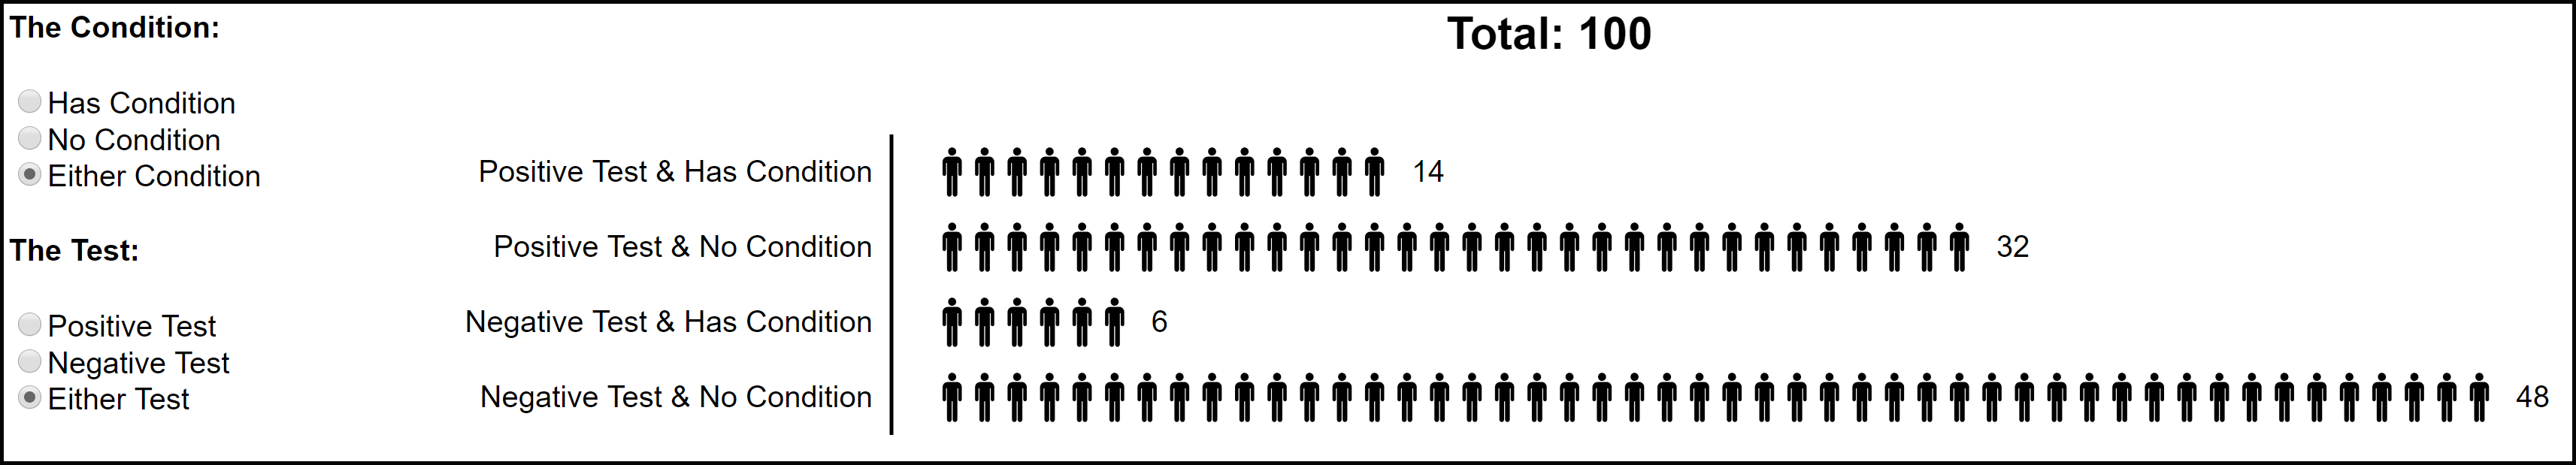
\includegraphics[width=\columnwidth]{img/teaser-EDIT.png}
    \caption{Interactive Visualization for Bayesian Statistics}
    \label{fig:interactive}
  \end{figure}
}

\newcommand\interactiveVisToggle{
  \begin{figure}
    \centering
    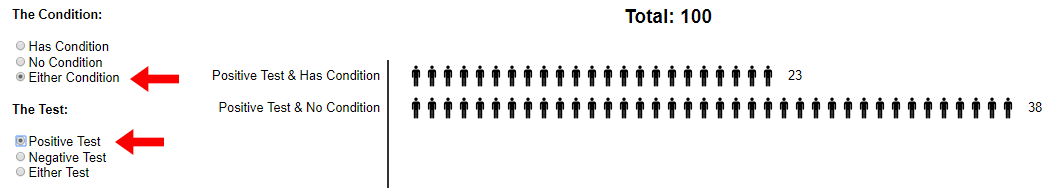
\includegraphics[width=\columnwidth]{img/interactive-toggle-EDIT.png}
    \caption{Interactive Visualization for Bayesian Statistics wit Condition Toggled On}
    \label{fig:interactive-toggle}
  \end{figure}
}

\newcommand\staticVis{
  \begin{figure}
    \centering
    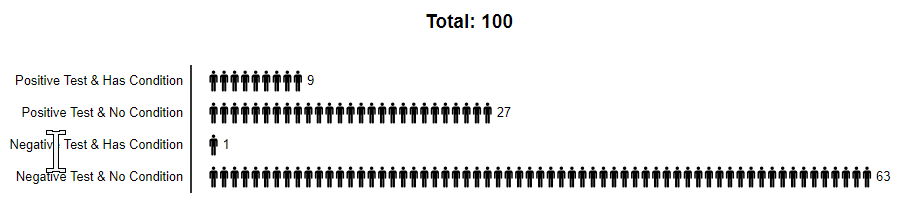
\includegraphics[width=\columnwidth]{img/static}
    \caption{Static Visualization for Bayesian Statistics}
    \label{fig:static}
  \end{figure}
}

% Import Tables
\newcommand\testtable{

\begin{table}[]
\centering

\begin{tabular}{r c c c c}

& \multicolumn{2}{c}{Our Results} & \multicolumn{2}{c}{Their Results} \\
\multicolumn{1}{l|}{\textbf{Measures}} & \textbf{Exp} & \textbf{Control} & \textbf{Control} & \textbf{Exp} \\ \hline
\multicolumn{1}{l|}{measure A}  & 54.8  & 48.6  & 44  & 33  \\ 
\multicolumn{1}{l|}{measure B}  & 32.2  & 28.8  & 8   & 6   \\ \hdashline
\multicolumn{1}{l|}{measure C} 	& 22.8  & 19.8  & 35  & 26  \\ 

\end{tabular}

\caption{As you can see, we are the best.}
\label{tab:results}
\end{table}

}


%% We encourage the use of mathptmx for consistent usage of times font
%% throughout the proceedings. However, if you encounter conflicts
%% with other math-related packages, you may want to disable it.

%% This turns references into clickable hyperlinks.
\usepackage[bookmarks,backref=true,linkcolor=black]{hyperref} %,colorlinks
\hypersetup{
  pdfauthor = {Saahil Claypool},
  pdftitle = {},
  pdfsubject = {},
  pdfkeywords = {},
  colorlinks=true,
  linkcolor= black,
  citecolor= black,
  pageanchor=true,
  urlcolor = blue,
  plainpages = false,
  linktocpage
}

%% If you are submitting a paper to a conference for review with a double
%% blind reviewing process, please replace the value ``0'' below with your
%% OnlineID. Otherwise, you may safely leave it at ``0''.
\onlineid{0}

%% declare the category of your paper, only shown in review mode
\vgtccategory{Evaluation}

%% allow for this line if you want the electronic option to work properly
\vgtcinsertpkg

%% In preprint mode you may define your own headline.
%\preprinttext{To appear in an IEEE VGTC sponsored conference.}

%% Paper title.

\title{The Effects of Interaction on Bayesian Reasoning}

%% This is how authors are specified in the journal style

%% indicate IEEE Member or Student Member in form indicated below
\author{Saahil Claypool, Claire Danaher, Alex Shoop}
\authorfooter{
%% insert punctuation at end of each item
\item
% Lane Harrison is with Worcester Polytechnic Institute. E-mail: [lane]@cs.wpi.edu.
 Saahil Claypool is a student at Worcester Polytechnic Institute. Email: [smclaypool]@cs.wpi.edu.
\item
 Alex
\item
 Claire
}

%other entries to be set up for journal
\shortauthortitle{Author \MakeLowercase{\textit{et al.}}: Title}

%% Abstract section.
\abstract{
Your abstract is great.
} % end of abstract

%% Keywords that describe your work. Will show as 'Index Terms' in journal
%% please capitalize first letter and insert punctuation after last keyword
\keywords{Perception, Visualization, Evaluation.}

%% ACM Computing Classification System (CCS). 
%% See <http://www.acm.org/class/1998/> for details.
%% The ``\CCScat'' command takes four arguments.

\CCScatlist{ % not used in journal version
 \CCScat{K.6.1}{Management of Computing and Information Systems}%
{Project and People Management}{Life Cycle};
 \CCScat{K.7.m}{The Computing Profession}{Miscellaneous}{Ethics}
}

%% Uncomment below to include a teaser figure.
% Teaser should be jnds for -pcp versus +pcp (distinguishable; not distinguishable; target; not distinguishable; distinguishable)
\teaser{
  \centering
  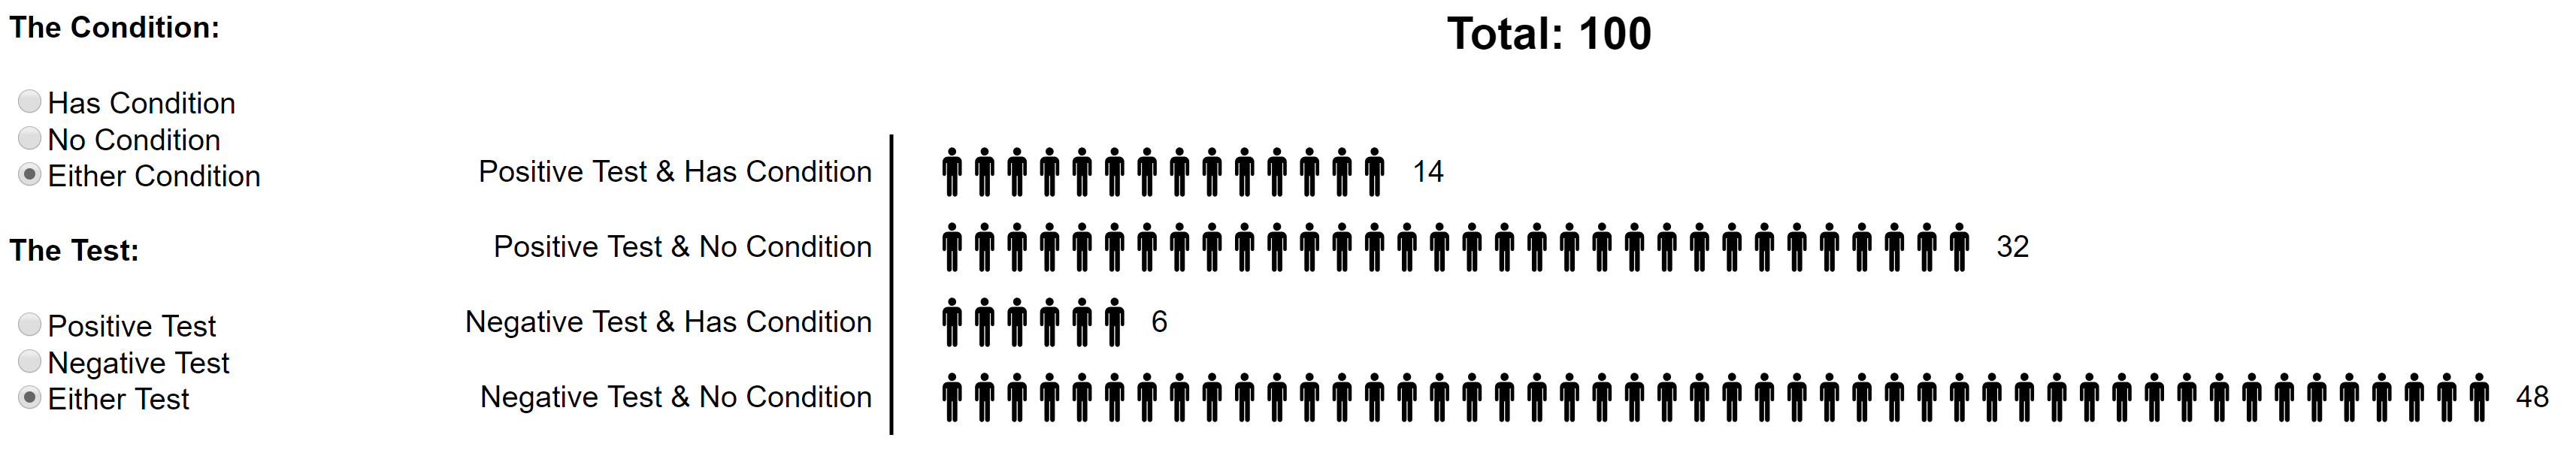
\includegraphics[width=\textwidth]{img/teaser.png}
  \caption{An Interactive Visualization for Bayesian Statistics}
  \label{fig:teaser}
}

%% Uncomment below to disable the manuscript note
%\renewcommand{\manuscriptnotetxt}{}

%% Copyright space is enabled by default as required by guidelines.
%% It is disabled by the 'review' option or via the following command:
% \nocopyrightspace

%%%%%%%%%%%%%%%%%%%%%%%%%%%%%%%%%%%%%%%%%%%%%%%%%%%%%%%%%%%%%%%%
%%%%%%%%%%%%%%%%%%%%%% START OF THE PAPER %%%%%%%%%%%%%%%%%%%%%%
%%%%%%%%%%%%%%%%%%%%%%%%%%%%%%%%%%%%%%%%%%%%%%%%%%%%%%%%%%%%%%%%%

\begin{document}

%% The ``\maketitle'' command must be the first command after the
%% ``\begin{document}'' command. It prepares and prints the title block.

%% the only exception to this rule is the \firstsection command
\firstsection{Introduction}

\maketitle

%% \section{Introduction} %for journal use above \firstsection{..} instead

% Introduction section is automatically added
% Hello World. Please see \S\ref{sec:conclusion}.

Advances in technology in the past decade have resulted in an exponential
growth in the amount of data being collected on a variety of topics. This has
lead to a movement towards using data driven decision making in increasingly
diverse arenas. Data is being used to make decisions ranging from the
potentially mundane, such as which individuals are qualified for an auto
loan, to the life altering, such as medical test results.

Past research has shown that even highly trained individuals are likely to
misinterpret statistical results. Consider the following standardized
statement about mammography screening results \cite{Ottley2016}:

\begin{displayquote}
    The probability of breast cancer is 1% for women at age forty who participate
    in routine screening. If a woman has breast cancer, the probability is 80%
    that she will get a positive mammography. If a woman does not have breast
    cancer, the probability is 9.6% that she will also get a positive
    mammography. A woman in this age group had a positive mammography in a
    routine screening. What is the probability that she actually has breast
    cancer? 
\end{displayquote}

Despite the seemingly routine nature of this question, research has shown
that many medical professional misinterpret these results leading to
potentially serious consequences such as over diagnosis \cite{Friederichs2014, Welch2010}. While
medical professionals are used in the previous scenario, research has shown
that most individuals lack a robust understanding of conditional
probabilities which impacts their ability to interpret results.

In the past, researchers have proposed ways to facilitate reasoning by
changing the presentation of the results. In research completed by Hoffrage
and Giegrenzer \cite{Gigerenzer1995}, the authors studied the comprehension benefits of
using frequency formats. They postulate that, when provided frequency data
rather than probabilities, medical professionals are better able to interpret
conditional probabilities. Further research by Harrison et. al. supports that
the presentation of information can have a significant positive effect on the
ability for people to reason about conditional probabilities \cite{Ottley2016}. Even with
these improvements, people still make many mistakes while reasoning about
these problems.

Similar to previous work, the aim of our research is to further explore
techniques for improving the presentation of Bayesian information to improve
reasoning. We postulate that, as suggested by previous work, an interactive
design will help problem solvers reason about conditional probabilities by
providing a 'guide' for reasoning about the problem \cite{Tsai2011}. Specifically, we

propose that an interactive frequency chart, where users can select or view
different conditions will reduce the information presented to a user and thus
help them complete a provided Bayesian reasoning problem.

To test this hypothesis, we conducted an experiment asking mechanical turk
participants to answer a Bayesian inference problem, similar to the one
stated above. We tested three different presentations of the conditional
probabilities: plain text, a static visualization, and an interactive
visualization. From this experiment, we were able to draw the following
conclusions:

\begin{itemize}
    \item As prior research indicates, people perform poorly on this seemingly simple Bayesian reasoning task. This is even true for users that claim a ‘high’ statistical familiarity.
    \item Interaction did not seem to have a positive effective on reasoning. In fact, there is some indication it caused users to perform worse on their reasoning task. We hypothesize this could be because it made the information more confusing or distracted the user. 
\end{itemize}



\guessAError

\section{Background}
Over the past three decades, research focused on understanding the cause of inaccuracy for both low and high numeracy individuals'
ability to interpret Bayesian Statistics. Lines of research include studies to
investigate the cognitive challenges associated with accurately interpreting
these types of statistics as well as whether or not visualization can help
overcome these challenges. 

Research conducted in the 1990s focused around the hypothesis that inclusion
of diagrams would help to improve users mental models whereby improving
accuracy. Research completed by Cole in 1989, suggested that the
inclusions of visualizations could improve interpretation \cite{Cole1989}. The study showed
that tendency towards over reliance on sensitivity (whereby influencing the
conclusions drawn) persisted despite verbal intervention and
training for participants tasked with interpreting written probabilistic
outcomes. However, this tendency decreased with the inclusion of a
frequentist visual representation. Cole attributes the difficulties of
interpretation without graphics to the lack of a mental model to support
understanding.

A study completed by Gigerenzer and Hoffrage \cite{Gigerenzer1995} illustrated the
underlying cognitive logic used by individuals to interpret Bayesian
statistics. This study found that calculations, when provided asked a problem about Bayesian reasoning, people were better able to interpret frequencies rather than probabilities. The researchers
hypothesized that this was a result of reduced cognitive load. The study showed that users were
approximately 30\% more likely to use Bayesian logic when presented with
frequency as opposed to probability information. Furthermore, the study
showed that with the use of frequency formats, the use of cognitive
algorithms became more consistent over time. Whereas there was little or no
improvement over time with the use of probability formats.

These results by Gigerenzer and Hoffrage \cite{Gigerenzer1995} align with the
previously completed work by Cole \cite{Cole1989}; participants were found to
perform better when they were provided with frequency formats over
probabilities. While Cole did not explicitly test frequencies against
probabilities hypothesis, numerical frequencies were presented visually for 3
out of the 4 diagrams used in Cole’s study. Participants showed improvements
with training with the use of visuals(frequencies) but found no improvement
with the use of standard probabilities. This improvement provided by frequency formats has been observed and confirmed in other studies in areas such as public health, psychology, and data visualization \cite{Eddy1982, Galesic2009, Cohen2007, Brown2014, Brase2009}. 

A number of studies have test the hypothesis that the inclusion of
visualization improves participant accuracy \cite{Brown2014, Friederichs2014,
Cohen2007}. The results of this work have been inconclusive. In a paper by
Ottley et al. \cite{Ottley2016}, the researchers parse through discrepancies
of past research by testing finely defined hypotheses pertaining to both
linguistic and visual representation of the information. For a detailed
discussion of discrepancies in past work please reference Ottley et al \cite{Ottley2016}.
Ottley’s findings supported the assertion that using frequencies as opposed to
probabilities improved accuracy. However, participant accuracy rates using
text only or visualization only outperformed those using text plus
visualization.

The focus of this new research is to determine whether the inclusion of
interaction can improve upon past accuracy rates. Evaluating the use of
interaction is a burgeoning topic in the data visualization community.
Bahador et al completed a paper in early 2018 focused on explore the effects
on accuracy of different interactive visual encodings. While this work is
somewhat tangential, the authors found that the use of position showed the
highest level of accuracy. Research completed by Tsai et al \cite{Tsai2011} failed to
produce statistically significant results however findings showed improvement
by users who used an interactive tool when compared to frequency and
probability only text.




\section{Methodology}
The methodology used for this research builds upon the methodology used by
Ottley et al.\cite{Ottley2016}. The test completed as part of this work 
linguistic comparison of text containing probabilities versus frequencies.
The findings were consistent with past studies and therefore this research
does not delve further on this topic. The second test completed focused on
the comparison text only, visualization only(vis only) and visualization and
text(vis+text). The results of this study showed that improvement was not
achieved through the inclusion of vis+ text when compared to vis only or text
only. Similar results have been found in other studies. This study builds
upon this past research by testing whether improvements can be achieved
through the use of interaction.

We recruited 80 participants using Amazon's Mechanical Turk (MTurk) service and supplemented these participants with our colleagues. Participants were directed to our survey via an external link and results were recorded on a server set up for this experiment. Each participant was given a unique verification code upon the completion of their task. 

Tree test cases were used in this study: text-only, vis-only, and interactive vis. The background text for all cases is as follows:

\begin{displayquote}
    There is a newly discovered disease, Disease X, which is transmitted by a bacterial infection found in the population. There is a test to detect whether or not a person has the disease, but it is not perfect. Here is some information about the current research on Disease X and efforts to test for the infection that causes it.
\end{displayquote}

The user is then presented with one of the three test cases as described in greater detail below. Users were selected at random as to which test case they were assigned. The numerical specifics that a user was presented with were randomly selected from a set of pre-selected test cases. All participants are then asked to answer the following questions:

‘100 people are tested for Disease X’:
\begin{enumerate}
    \item How many people do you think will test positive?
    \item Out of those people, how many will have the disease? 
\end{enumerate}

\subsection{Design 1: Text-Vis}
As previously mentioned, the baseline case was designed to match the language used by Ottley et al. \cite{Ottley2016}. A sample of the textual statement is as follows:

\begin{displayquote}
    There is a total of 100 in the population. Out of the 100 people in the population,20 people actually have the disease. Out of these 20 people, 14 will receive a positive test result and 6 will receive a negative test result. On the other hand, 80 people do not have the disease (i.e., they are perfectly healthy). Out of these 80 people, 8 will receive a positive test result and 72 will receive a negative test result.
\end{displayquote}

This description is a combination of the main components of a good text representation, those being framing, narrative, and probing.

\subsection{Design 2: Vis-Only}

\staticVis

For the vis-only test case, pictorial representation (human-like figures) were used to show the frequency count of tested/conditioned members of the population. Figures were shown along a horizontal axis, grouped along the vertical axis by the specific attribute: ‘positive test and has condition’, ‘positive test and no condition’, ‘negative test and has condition’, and ‘negative test and no condition.’ An example arrangement can be seen in \ref{fig:static}. 

\subsection{Design 3: Interactive-Vis}

\interactiveVis

\interactiveVisToggle

We implemented interactivity using the same pictorial representation as the
vis-only representation. The interactive vis tool includes selectable buttons
on the left-hand-side of the chart. Participants can use the selectable
buttons to toggle through different scenarios. For example if a user toggles
on the ‘Has Condition’ button, the pictorial representation changes to only
show the people icons associated with ‘positive test and has condition’ and
‘negative test and has condition.’ Transitions and animation were included
for inverse selection. For example, if a user toggled of the ‘No Condition’
button, icons were removed from the screen. The figures below show a static
view of interactive states. Figure \ref{fig:interactive} shows the starting screen for the
interactive visualization tool. Figure \ref{fig:interactive-toggle} is an example of toggling the button
to specify the selection to answer the second lab question.


\section{Results}

\demographicstable

\accuracyPlot

\educationAccuracy

\experienceAccuracy

\guessAError

A total number of 104 individuals participated in the experiment. The
distribution of participants by group are 30, 38 and 36 completes for
text-only, vis-only and interactive responses respectively. Demographic
information was collected as part of the experiment. A summary of demographic
information of our experiment participants can be found in Table \ref{tab:demographics}.

For the purposes of this analysis, responses were characterized using a
binary approach of either correct or incorrect. So for our overall
experiment, only 50 of the 104 participants were correct (48\% accuracy). The
overall accuracy across each visualization type was also observed.The
logarithmic (base 2) error score was calculated for both of the two
experiment questions, as seen in Figure \ref{fig:accuracyPlot}.

We also observed how the results looked when separated by the educational
background and statistical understanding for each of the participants. The
results of which can be found in Figure \ref{fig:educationAccuracy} and Figure \ref{fig:experienceAccuracy} respectively.

A chi-squared test was conducted across all participants and discovered a
not-so-significant value when trying to see if there were significant
differences between the accuracy rates and visualization type $\chi^2$(df = 2, N = 100)=2.1991, p = 0.333). Furthermore,
performing pairwise chi-square tests on each pairing also did not show any
significance; between vis-only and text, ($\chi^2$(df = 2, N = 68)=0.26845, p =
0.8744), between interactive and text ($\chi^2$(df = 2, N = 66)=1.9683, p =
0.3738), and between interactive and vis-only ($\chi^2$(df = 2, N = 74)=2.9178,
p = 0.2525.



\section{Discussion}
The purpose of this experiment was to test whether participants would more
accurately interpret statistics when the results were presented as an
interactive visualization tool. The baseline method for this experiment was
to ask participants to interpret questions phrased as frequencies. This
baseline was adapted from the text used by Ottley. We did not observe
statistically significant results for the differences between the text-only,
vis-only and interactive vis test cases. Therefore,we cannot conclude that
interaction had any positive effect on the accuracy of the participants
Bayesian reasoning. In fact, the group that received the interactive
visualization performed slightly worse (although not a statistically
significant amount). This may indicate that the interaction added an
additional layer of complexity and hindered the user's performance. These
trends were echoed verbally by users included in an initial pilot study. But,
a follow up study with more users would be needed to confirm this.

The results produced by this study align with findings by Ottley where the
vis-only and text-only results produced statistically similar accuracy rates.
The accuracy rates of approximately 50\% for the vis-only case aligned are
slightly higher rate of 40\% as observed by Metcalfe Et Al. The 40\% accuracy
rate for the text-only case are lower than those observe by Ottley. However,
the sample size for this group was slightly smaller and the difference was
not observed to be statistically significant. Therefore, the difference is
likely attributable to aberrations due to the smaller sample size.

Interestingly, accuracy rates for those who self identified as having low
numeracy skills increased between the text-only, vis-only and interactive vis
respectively. This same trend was not observed for medium and high numeracy
participants. An area for potential future research could be further
exploring the relationship between numerical literacy and accuracy rates
between cases.


\section{Conclusion}
\label{sec:conclusion}
As statistics become increasingly pervasive as a tool in decision making for
people of all numeracy skill levels, the need for effectively expressing this
information grows. The focus of this research was to determine whether the
inclusion of interaction could be used to improve interpretation accuracy
rates. The experiment did not produced statistically significant difference
between text-only, vis-only and interactive-vis test cases. However, our
findings aligned with past studies and can serve as a foundation for future
work on the effects of interaction and statistical reasoning.

%% if specified like this the section will be committed in review mode
\acknowledgments{
Text.
}

\bibliographystyle{abbrv}
\bibliography{paper}


\end{document}
